\documentclass[a4paper]{article}
\usepackage[utf8]{inputenc}
\usepackage[T1]{fontenc}
\usepackage{cite}
\usepackage{graphicx}
\usepackage{hyperref}

\iffalse
1) Le contexte, la problèmatique, les contributions de l’article choisi (2 pages environ)
2) Le plan d’expérience que vous comptez mener, les données que vous comptez utiliser (2 pages max).
\fi

\title{Projet AS : WaveNet}
\author{Seurin Mathieu}

\begin{document}

\maketitle

\section{WaveNet : Génération de son}

Le but de WaveNet \cite{wavenet}, à la base, est de faire de la génération de son brut et plus particulièrement la génération de voix humaine (on verra que WaveNet va plus loin). L'idée est simple, le programme reçoit en entrée un texte, et le but est de faire sortir une voix la plus réalise possible, récitant le texte. Cette tâche s'appelle de la synthèse vocal ou TTS (Text-To-Speech).

Il existe deux concurrents actuellement et c'est avec eux que WaveNet est comparé. Le premier s'appelle 'concatenative TTS' (méthode par concatenation) et le deuxième 'parametric TTS' (méthode paramétrique). La méthode par concatenation utilise pleins d'enregistrements de voix et les 'colle' bout à bout pour générer le discours mis en entrée. Le processus fonctionne relativemment bien mais il a ses limites. L'enregistrement est coûteux car il faut le faire pour chaque mot (et rajouter un mot nécessite un nouvel enregistrement) et l'enregistrement doit être très precis (même timbre de voix, même vitesse de parole, même volume etc ...). De plus, ajouter une nouvelle voix oblige à ré-enregistrer tout. La deuxième méthode est paramétrique : Au lieu de coller des enregistrements de mots, le discours va être généré par le modèle. Les premiers sont des modèles dits de vocodeur, où on va appliquer plusieurs filtres sur un signal pour simuler l'appareil vocal d'un humain et donc simuler une voix.
Les deuxièmes sont des modèles qui auront appris sur une base de voix humaine (WaveNet rentrent dans cette catégorie, de modèles appris sur de la voix humaine). Classiquement ces modèles sont à base de chaines de Markov.

La problématique est d'obtenir un son de voix qui est le plus naturel possible et avoir des modèles flexibles. Les modèles par concatenation sonnant relativement bien, parfois un peu haché, mais ils ne sont pas du tout flexible. Actuellement les modèles paramétriques sont plus flexible, mais sonne moins naturel que les méthodes par concatenation.
L'objectif de WaveNet est donc de créer un modèle paramétrique flexible et qui soit au moins aussi bon que des modèles par concatenation.

\section{L'approche de WaveNet}

L'approche WaveNet est celle d'un modèle paramétrique, avec base d'apprentissage. Pour le moment, la littérature est centrée sur des modèles RNN et LSTM \cite{DBLP:journals/corr/ZenAEHS16}., mais on trouve également des modèles Markoviens \cite{Raitio:2011:HSS:2209821.2210690}.

L'approche WaveNet est à base de réseaux de neurones convolutifs causaux dilatés. Nous allons expliquer le principe plus en détails.

Le but est de générer un signal d'environ 16000 échantillons à la seconde, chaque échantillon dépendant des échantillons précédents (on verra dans quel mesure).
L'architecture proposée n'est pas à base de RNN mais de réseaux de convolutions causaux, ce qui veut dire que l'output $x_t$ (échantillon $x$ au temps $t$) va être la résultante de filtres de convolution appliqués au $x_k ... x_{t-1}$ avec $k<t$ (voir \autoref{fig:SimpleModel}, où sont utilisées 3 couches de convolution pour illustrer, dans la réalité, il y a bien plus de couches et les filtres sont plus gros)

\begin{figure}[h]
  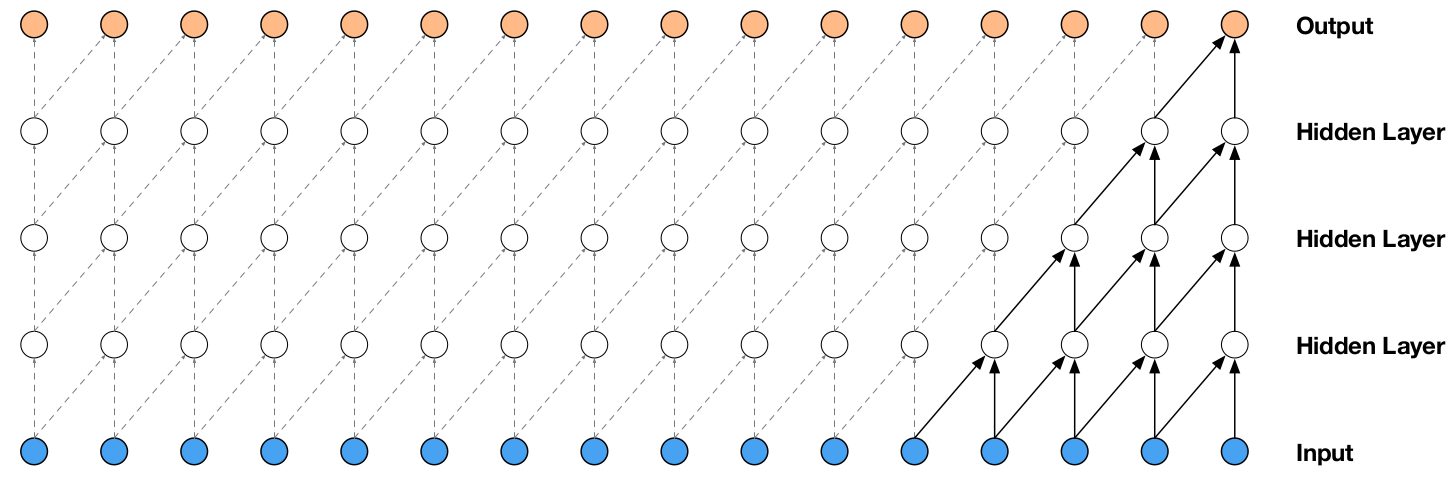
\includegraphics[scale=0.2]{modelSimple.png}
  \caption{\label{fig:SimpleModel} Réseaux de convolutions causaux}
\end{figure}

Le principal problème de cette architecture est qu'elle a besoin d'énormément de couches (combinaisons de plusieurs filtres) et de filtres gros (= qui filtrent beaucoup de pas de temps et qui remonte loin dans le passé), cela pose donc un problème niveau temps/coût de calcul.

Pour remédier au deuxième problème, les auteurs utilisent une structure différente : Les CNN causaux dilatés. Le principe est illustré sur la \autoref{fig:modelDilate}. Le but est d'augmenter la taille des filtres des couches cachées mais sans décupler le nombre de calcul à effectuer. Cela permet aux filtres des couches cachés de récupérer de l'infos de pas de temps plus éloignés.

Plus l'on va dilater un filtre, plus il va capter l'information de pas temps éloignés. Attention, un fitre trop dilaté risque de 'sauter' des pas de temps et d'ignorer les échantillons récents, ce qui n'est pas un comportement voulu.

\begin{figure}[h]
  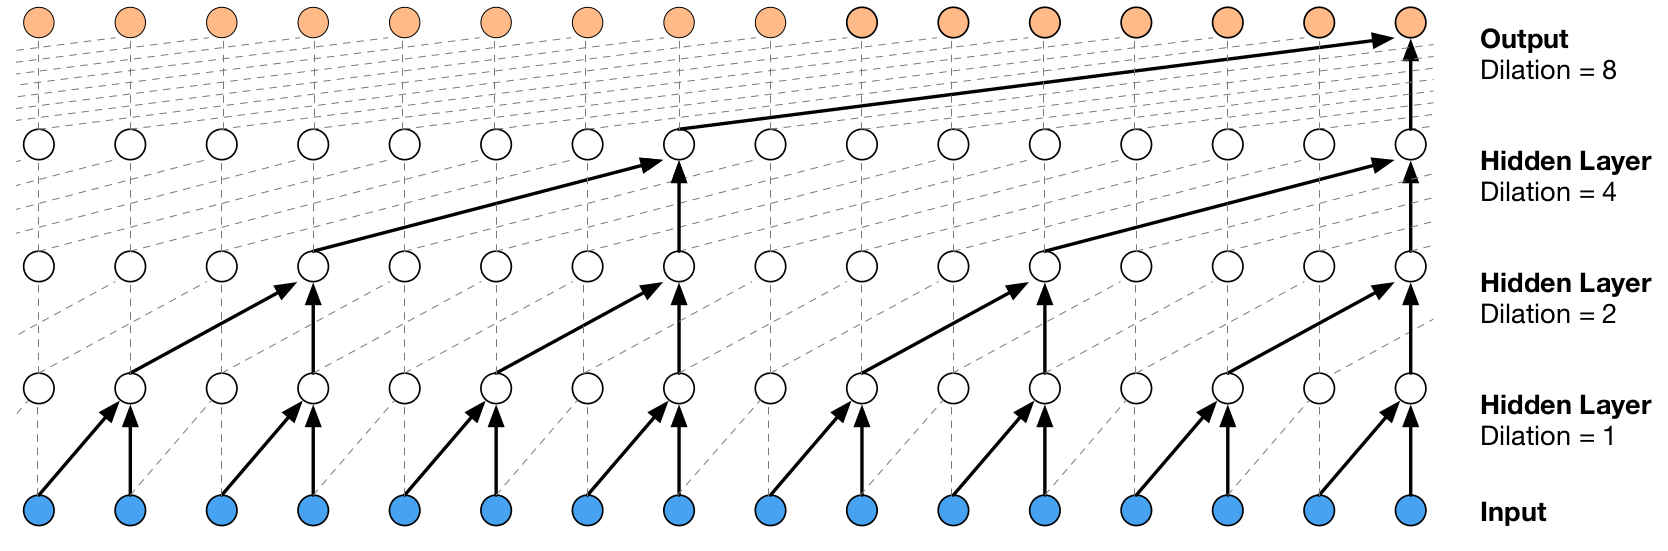
\includegraphics[scale=0.2]{modelDilate.png}
  \caption{\label{fig:modelDilate} Réseaux de convolutions causaux}
\end{figure}

\section{Expériences mises en place}

L'application de WaveNet est évidemment la génération de voix humaine, mais nous avons détourné son utilisation pour en faire un générateur de musique midi. WaveNet permet de générer du son mais représente 60h de base d'entrainement, apprise pendant plusieurs semaines sur (multiples) GPU. Il génère 16 000 échantillons à la seconde (et cela prend 90 minutes pour générer une seconde de son), tous ces chiffres pour dire : Générer du son, c'est une structure hors-norme et donc impossible à reproduire sans des moyens. Donc, on va générer de la musique MIDI (car même si le tempo est élevé, il y rarement plus de 16000 notes à la seconde)

WaveNet se décompose donc en deux phases : (Apprentissage et prédiction)
\begin{enumerate}
\item En apprentissage : L'entrée est une série de notes et la sortie un ensemble de vecteur de probas (si on produit 2 notes en sortie, on aura donc 2 vecteurs de distributions de probas). Le nombre de sorties dépend du nombre de couches, de la taille des filtres et du nombre d'entrée. 

\item En génération : L'initialisation se fait avec une séquence de notes (généralement de la base d'entrainement). En sortie, on obtient une distribution de probabilités selon laquelle est tirée une note. Cette note est ensuite rajoutée à la fin de la séquence et on réitère le processus autant de fois que l'on veut de notes.
\end{enumerate}

La structure de WaveNet reproduite ici est la structure de base. C'est à dire des couches de convolutions empilées, avec un filtre de taille 2 (chaque noeud filtre un pas de temps et son prédecesseur) et un stride de 1 (Chaque couche prend n entrées et produit n-1 sorties).

Le calcul pour le nombre de sorties en fonction du nombre d'entrées est donc très simple :
$$\textrm{Nombre d'entrées} - \textrm{Nombre de couches de convolutions} = \textrm{Nombre de sorties}$$

Il est important de noter qu'avec cette structure, le nombre de pas de temps dans le passé pris en compte par WaveNet est complètement déterminé par le nombre de couches de convolutions. Si on a deux couches, on prend en compte 3 pas de temps (2 + 1)

\subsection{Représentation des données}

Pour représenter la musique comme une structure qui puisse être apprise par WaveNet, il a fallu changer les musiques en elles-mêmes. Plusieurs choix ont été faits, et ils vont considérablement impacter la musique produite :
\begin{enumerate}
\item Une note est un vecteur de taille 128 (128 note possibles en MIDI) avec des zéros partout sauf à la case $i$ où un 1 est présent pour indiquer quelle note est jouée.
\item Transformer tous les accords (plusieurs notes jouées au même pas de temps) en prenant juste la fondamentale (note la plus importante de l'accord). Pourquoi faire cela ? Car la façon dont est construit WaveNet, il ne peut prédire qu'une seule note par pas de temps (l'output est un vecteur de probabilités) donc, on doit faire en sorte d'avoir des notes uniques en entrée et en sortie.
\item Normalement, dans la musique, la durée des notes est variable, il n'y a donc pas forcément une note jouée par pas de temps, juste une note qui dure. Pour arriver à représenter une note qui dure, on va découper chaque mesure en 32 pas de temps. Ainsi une noire (un quart de mesure) représentera 8 pas de temps, on va donc répéter la note 8 fois. Le gros problème de cette représentation est que l'on ne fait pas la différence, par exemple, entre deux blanches successives et 4 noires successives puisqu'elles vont être représentées de la même façon. \autoref{fig:noteRepr}
\end{enumerate}

\begin{figure}[ht]
  \caption{Les deux premières mesures seront donc réprésentées de la même façon, comme la dernière mesure}
  \includegraphics[scale=0.4]{noteRepr.png}
  \label{fig:noteRepr}
\end{figure}

Le dernier choix est particulièrement contraignant sur la musique, car il oblige au modèle d'aller capter des pas de temps très éloignés pour tenir compte des notes (voir des mesures) précédentes.

\subsection{Critère d'évaluation}

L'évalutation de modèle génératif n'est pas simple, car il serait nécéssaire de connaître la distribution sous-jacente à nos données, ce qui est impossible. Donc de façon générale, l'évaluation dépend de la tâche considérée. En musique, plusieurs critères sont possibles, nous avons choisi d'en traiter deux.

\subsubsection{Critère de dissonance}

Le principe serait le suivant : Il faut une cohérence au sein d'une mesure, c'est à dire que toutes les notes de cette mesure doivent bien sonner entre elles. Ceci en musique est défini par une gamme. Donc si toutes les notes au sein d'une mesure font partie de la même gamme, alors il y a cohérence (et donc pas de dissonance). À l'inverse, si des notes sortent de la gamme, alors elles seront dissonantes, et donc le modèle va être considéré comme moins bon.

Un premier critère peut donc être de compter le nombre de notes dissonantes sur la partiton générée.


\subsubsection{Critère de créativité}

Un critère de créativité a été proposé par \cite{hadj16} pour l'évaluation de modèle génératif en musique. Le principe est simple, un bon modèle génératif en musique est capable :

\begin{enumerate}
\item De retrouver des séquences qu'il a vu pendant les entraînements
\item De trouver de nouvelles séquences jamais vues en entrainement.
\end{enumerate}

Pour \cite{hadj16}, il était question des générations d'accords en musique, mais cette mesure peut-être adaptée pour la génération de musique de façon plus générale en regardant des séquences de n-grams (3-4 par exemple)
Ainsi, on a une idée de la capacité du modèle à apprendre des séquences et en plus de sa capacité à généraliser.

\subsection{Expériences sur données jouets}\label{sec:playground}

Dans un premier temps le but est de savoir si WaveNet est capable de capter des séquences de notes simples, avant de passer sur des séquences plus complètes voir des musiques entières.
Le but de cette partie était de vérifier que déja, le modèle fonctionnait bien, et de tester un peu ces limites.

La première séquence correspondait à une alternance de 'mi' et 'la' et en seulement quelques itérations, un modèle avec une couche de convolution arrive à apprendre la séquence sans souci.

La séquence étant extrêmement simple, il fallait tester sur une séquence un peu plus compliqué pour tester les limites du modèle.

\begin{figure}[ht]
  \caption{La séquence n'est pas beaucoup plus compliquée, mais elle permet d'illustrer un peu les limites du modèle actuel}
  \includegraphics[scale=0.30]{seq2.png}
  \label{fig:noteRepr}
\end{figure}

Encore une fois, la séquence n'est pas très compliquée, et en quelques itérations, un modèle avec deux couches apprend la séquence. Seulement, on commence à voir certaines limites quand on passe avec plus de couches.

Pour augmenter la portée de notre modèle dans le temps, il faut augmenter le nombre de couches. Or au bout de 9-10 couches, le modèle n'apprend absolument pas car le gradient diminue complètement et n'arrive pas à être propager jusqu'aux premières couches. On doit donc se restreindre moins de 9 couches avec l'architecture actuelle.

\subsection{Données réelles : Musique flamenco à la guitare}

Les données utilisées pour la suite sont des musiques de flamenco à la guitare par Paco DeLucia, les partitions MIDI sont disponible ici : \href{http://www.classicalguitarmidi.com/}{Classical Guitar Midi}

On va donc utiliser l'architecture pour apprendre sur une base de 6 chansons de DeLucia, et voir si le modèle arrive à retrouver le chanson et à générer des mélodies.

Avec 8 couches de convolution, on arrive à un score de 0.40 de précision (attention, ce score est celui obtenu sur la base d'entrainement, le score n'est donc pas forcément représentatif d'un bon modèle, il donne juste une idée de l'apprentissage du modèle mais aucunement de sa capacité à généraliser)

Le tableau récapitulatif est ici : \autoref{tab:filter2}

\begin{table}[ht]
  \centering
  \caption{Tableau de résultat avec filtre de taille 2 en fonction du nombre de couches}
  \label{tab:filter2}
  \begin{tabular}{lllll}
    Nombre de couches           & 2    & 5 & 8  & 12 \\
    Pas de temps pris en compte & 3    & 6 & 9  & 13 \\
    Score Accuracy              & 0.82 & 0.40  & 0.40 & 0.14   
  \end{tabular}
\end{table}

Premier constat, il est étonnant que le modèle avec deux couches arrivent très bien à prédire les notes futures alors qu'un modèle plus complexes y arrive moins bien.
Une explication probable est que de part la construction des nos données, les notes ont tendances à se répéter énormément, et donc, pour prédire, il suffit de prédire que la note suivante est la même que la précédente et on obtient des scores proches de 80\%. Pour pouvoir augmenter la précision de notre modèle, il faudrait que le modèle puisse prendre des pas de temps bien plus éloignés. Or le problème est que l'on a vu \autoref{sec:playground} que le gradient n'arrive pas à se propager au delà de 9 couches.

On constate qu'avec des filtre un peu plus gros, le constat est le même \autoref{tab:filter3}
\begin{table}[ht]
  \centering
  \caption{Tableau de résultat avec filtre de taille 3, les résultats ne changent pas beaucoup}
  \label{tab:filter3}
  \begin{tabular}{llll}
    Nombre de couches           & 1    & 7  & 12 \\
    Pas de temps pris en compte & 3    & 9  & 14 \\
    Score Accuracy              & 0.84 & 0.32 & 0.11   
  \end{tabular}
\end{table}

Les partitions produites sont d'ailleurs assez folkloriques :

\begin{figure}[ht]
  \caption{Partition produite avec le modèle à 6 couches}
  \includegraphics[scale=0.60]{seq6.png}
  \label{fig:part6}
\end{figure}

Par contre, un bon point est qu'il réussir à capter la clef dans laquelle se trouve la chanson et utilise des notes qui sonne bien ensemble, c'est le rythme et l'enchaînement qui n'est pas bon du tout.

\section{Conclusion et Perspectives}

On constate que le modèle en l'état ne permet pas d'apprendre correctement et de générer de la musique pour deux raisons :
\begin{enumerate}
\item La représentation des données ne semble pas adaptée
\item La structure actuelle ne permet pas la superposition de beaucoup de couches et donc de prendre en compte des pas de temps éloignés.
\end{enumerate}

Il faut donc réussir à capter des pas de temps plus éloignés et que le gradient se propage mieux. Pour cela, il y a deux stratégies:
\begin{enumerate}
\item Ajouter de la dilatation à notre modèle comme décrit \autoref{fig:modelDilate}
\item Ajouter des parties de 'skip-connection' c'est à dire créer des connections qui 'sautent' certaines couches, cela permet d'envoyer l'input directement à des couches plus profondes et permettre une meilleure propagation du gradient
\end{enumerate}

Pour aller plus loin, il faudrait pouvoir gérer les accords, à la fois en entrée mais surtout en sortie.

\bibliography{SeurinRapport}
\bibliographystyle{apalike}
\end{document}


